 \begin{center}\begin{large} Practice Problems 3
 \end{large}\end{center}

% 1 eigens
\begin{problem}
    Find the eigenvectors and the eigenvalues of the following matrix.
    \[
    \begin{bmatrix}
        -6 && 3 \\
        4 && 5
    \end{bmatrix}
    \]
    % https://www.mathsisfun.com/algebra/eigenvalue.html
\end{problem}

% 2 Limits
\begin{problem}
   Find, if exists, the limit of the sequence, as $n\to\infty$:

    \begin{enumerate}
        \item[a) ] $\dfrac{1}{n^2}$,
        \item[b) ] $\dfrac{n^2}{2-n^3}$,
        \item[c) ] $(0.99)^n$,
        \item[d) ] $(1.11)^n$,
        \item[e) ] $\sin {\pi n}$,


    \end{enumerate}
    Which of the sequences above are convergent?
\end{problem}

% 3 Derivatives
\begin{problem}
Calculate $f'(x)$:
    \begin{enumerate}
        \item[a) ] $x^2+4 $,
        \item[b) ] $3x^4-\dfrac{1}{x}$,
        \item[c) ] $5\sin^2 x$,
        \item[d) ] $xe^x$,
        \newpage
        \item[e) ] $\dfrac{2x-3}{4-x^3}$,
    \end{enumerate}
\end{problem}

% 4 Critical points
\begin{problem}
    \begin{figure}
        \centering
        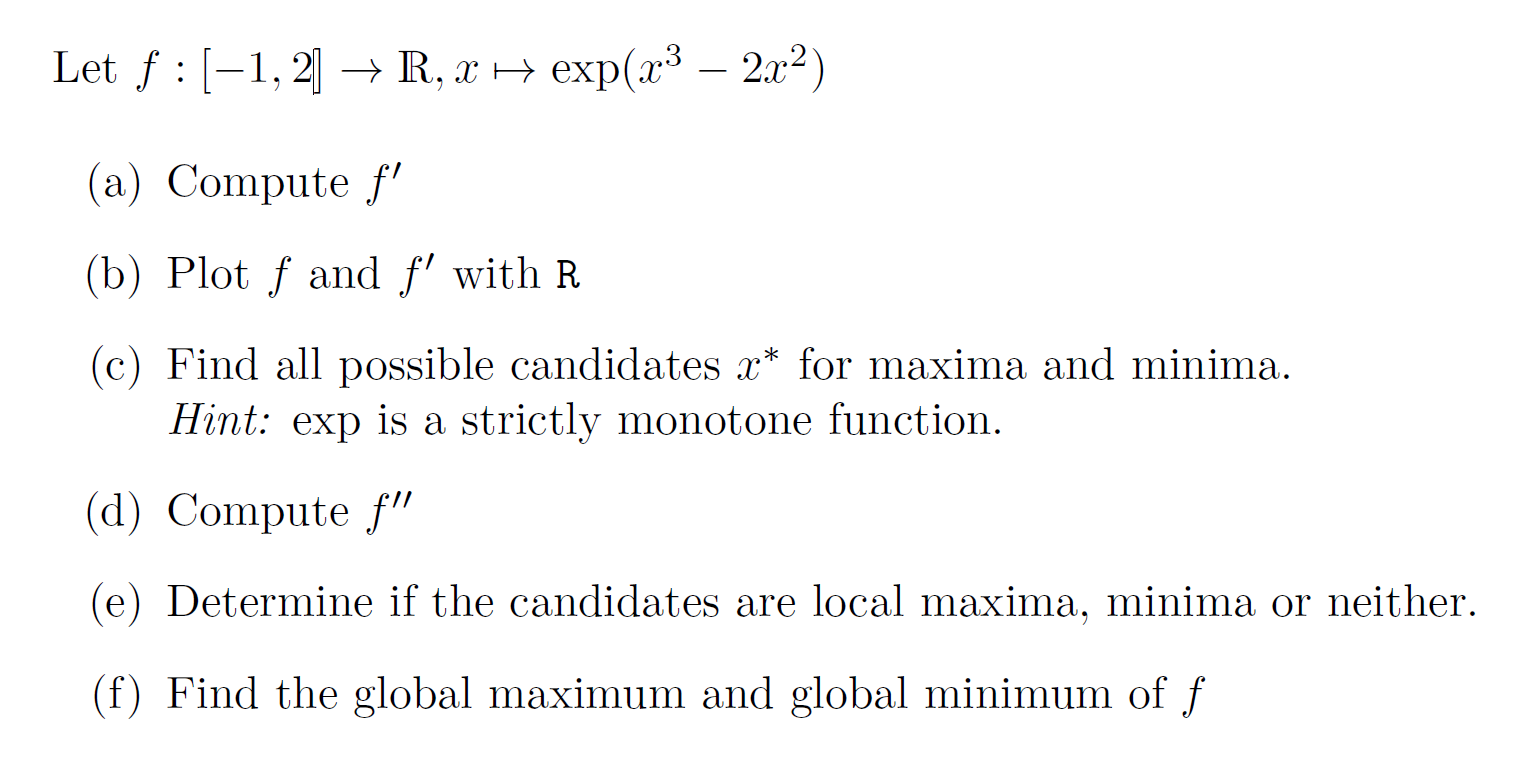
\includegraphics[width=1\linewidth]{figs/critical_points.png}
    \end{figure}
\end{problem}

% 5 Taylor
\begin{problem}
    \\
    \begin{enumerate}
        \item[a) ] Find the Taylor polynomial for the function $\cos{x}$, around point $x=0$
        \item[b) ]  Find the 3-rd order Taylor polynomial for the function $f(x) = \sqrt{x}$ centered at $x_0 = 9$
    \end{enumerate}
\end{problem}

% 6 Convexity
\begin{figure}
    \centering
    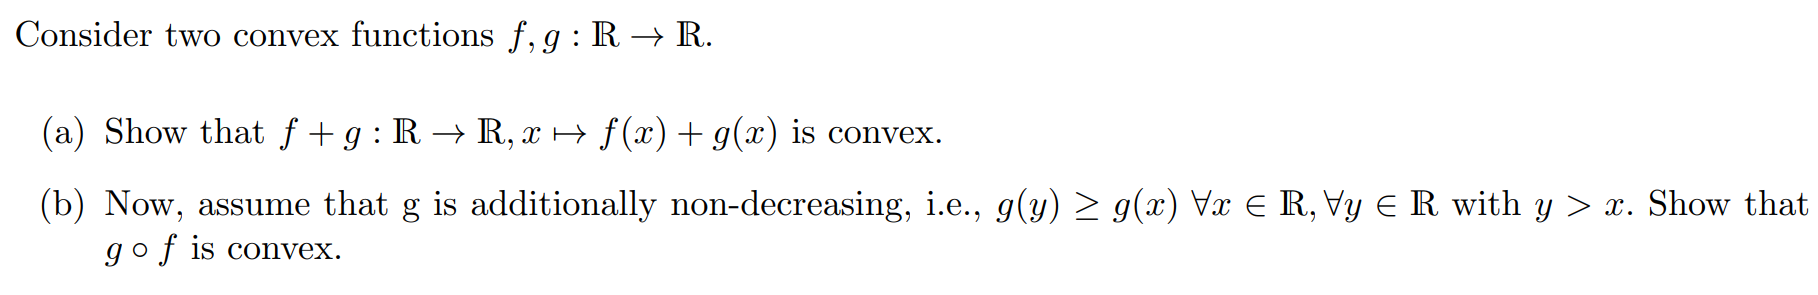
\includegraphics[width=1\linewidth]{figs/convexity.png}
\end{figure}